\documentclass[tikz,border=14pt]{standalone}
\usepackage{tikz}
\usepackage{amsmath}
\usepackage{amssymb}
\usetikzlibrary{arrows.meta,fit,backgrounds}

%% Color palette
\definecolor{cIn}   {RGB}{60,  60,  60}
\definecolor{cEnc}  {RGB}{50, 100, 185}
\definecolor{cMoE}  {RGB}{120, 45, 175}
\definecolor{cFus}  {RGB}{185, 45,  45}
\definecolor{cUAMM} {RGB}{40,  145, 70}
\definecolor{cAMF}  {RGB}{220, 110, 20}
\definecolor{cAux}  {RGB}{90,  160, 220}
\definecolor{cOra}  {RGB}{35,  130, 60}
\definecolor{cMI}   {RGB}{150, 50, 180}
\definecolor{cLoss} {RGB}{185, 45,  45}

\tikzset{
  BOX/.style   = {draw, very thick, rounded corners=5pt,
                  text centered, font=\small},
  inp/.style   = {BOX, fill=cIn!10,   draw=cIn!55,
                  minimum width=30mm, minimum height=11mm},
  enc/.style   = {BOX, fill=cEnc!12,  draw=cEnc!65,
                  minimum width=40mm, minimum height=28mm},
  fus/.style   = {BOX, fill=cFus!10,  draw=cFus!70,
                  minimum width=44mm, minimum height=42mm},
  wgt/.style   = {BOX, fill=white,    draw=gray!50,
                  minimum width=36mm, minimum height=11mm, font=\scriptsize},
  trk/.style   = {BOX, fill=cUAMM!10, draw=cUAMM!65,
                  minimum width=36mm, minimum height=30mm},
  amf/.style   = {BOX, fill=cAMF!12,  draw=cAMF!75,
                  minimum width=30mm, minimum height=18mm},
  aux/.style   = {BOX, fill=cAux!12,  draw=cAux!65,
                  minimum width=36mm, minimum height=18mm},
  ora/.style   = {BOX, fill=cOra!10,  draw=cOra!65,
                  minimum width=30mm, minimum height=18mm},
  lss/.style   = {BOX, fill=cLoss!8, draw=cLoss!60,
                  minimum width=60mm, minimum height=18mm},
  mib/.style   = {BOX, fill=cMI!8,   draw=cMI!60,
                  minimum width=60mm, minimum height=20mm},
  trBox/.style = {draw=gray!40, dashed, rounded corners=6pt,
                  fill=gray!3, inner sep=8pt},
  A/.style     = {-Stealth, very thick, line width=1.1pt},
  Ad/.style    = {-Stealth, thick, dashed, opacity=0.6},
  PL/.style    = {font=\normalsize\bfseries},
}

\begin{document}
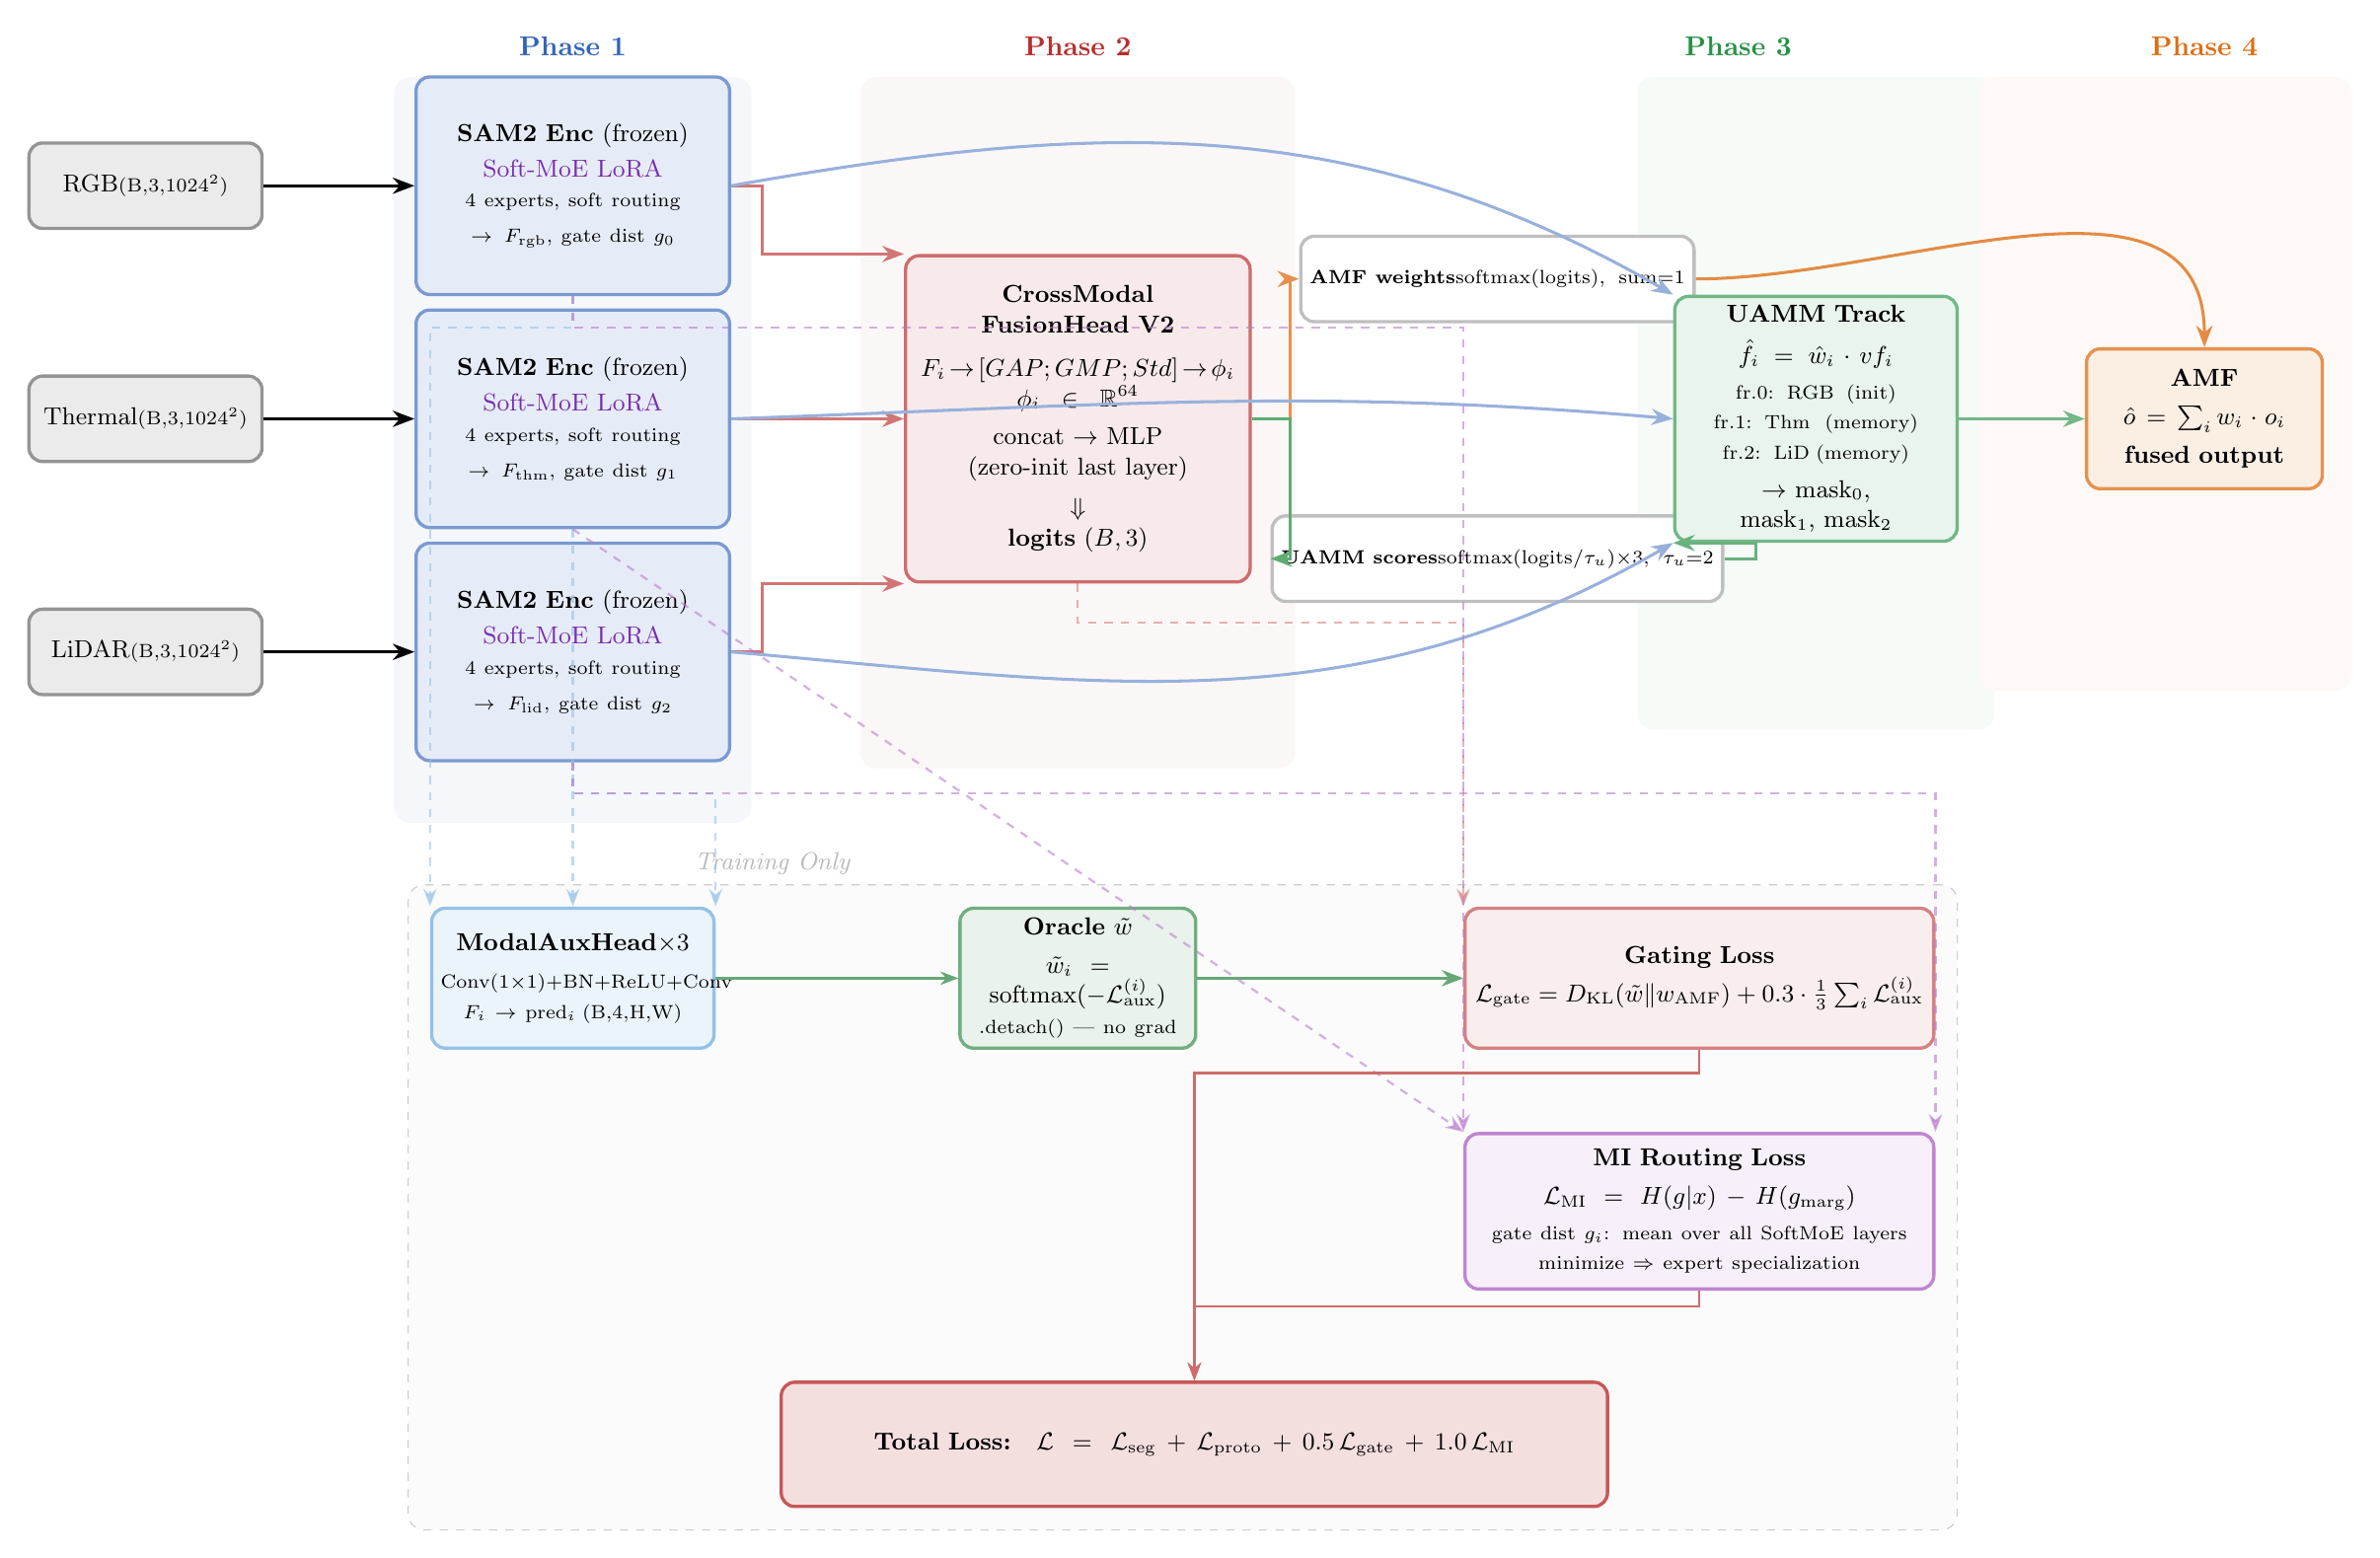
\begin{tikzpicture}

%% ────────────────────────────────────────────────────────────
%%  PHASE LABELS
%% ────────────────────────────────────────────────────────────
\node[PL, text=cEnc]  at ( 5.5, 4.8) {Phase~1};
\node[PL, text=cFus]  at (12.0, 4.8) {Phase~2};
\node[PL, text=cUAMM] at (20.5, 4.8) {Phase~3};
\node[PL, text=cAMF]  at (26.5, 4.8) {Phase~4};

%% ────────────────────────────────────────────────────────────
%%  COLUMN 0: Raw Inputs  (x=0)
%% ────────────────────────────────────────────────────────────
\node[inp] (iR) at (0,  3.0) {RGB\\{\scriptsize(B,3,1024$^2$)}};
\node[inp] (iT) at (0,  0.0) {Thermal\\{\scriptsize(B,3,1024$^2$)}};
\node[inp] (iL) at (0, -3.0) {LiDAR\\{\scriptsize(B,3,1024$^2$)}};

%% ────────────────────────────────────────────────────────────
%%  COLUMN 1: SAM2 Encoders + Soft-MoE LoRA  (x=5.5)
%% ────────────────────────────────────────────────────────────
\node[enc, text width=38mm] (eR) at (5.5,  3.0)
  {\textbf{SAM2 Enc} (frozen)\\[2pt]
   {\color{cMoE}\small Soft-MoE LoRA}\\
   {\scriptsize 4 experts, soft routing}\\[2pt]
   {\scriptsize $\to F_\text{rgb}$, gate dist $g_0$}};
\node[enc, text width=38mm] (eT) at (5.5,  0.0)
  {\textbf{SAM2 Enc} (frozen)\\[2pt]
   {\color{cMoE}\small Soft-MoE LoRA}\\
   {\scriptsize 4 experts, soft routing}\\[2pt]
   {\scriptsize $\to F_\text{thm}$, gate dist $g_1$}};
\node[enc, text width=38mm] (eL) at (5.5, -3.0)
  {\textbf{SAM2 Enc} (frozen)\\[2pt]
   {\color{cMoE}\small Soft-MoE LoRA}\\
   {\scriptsize 4 experts, soft routing}\\[2pt]
   {\scriptsize $\to F_\text{lid}$, gate dist $g_2$}};

\draw[A] (iR)--(eR);
\draw[A] (iT)--(eT);
\draw[A] (iL)--(eL);

%% ────────────────────────────────────────────────────────────
%%  COLUMN 2: CrossModalFusionHeadV2  (x=12)
%% ────────────────────────────────────────────────────────────
\node[fus, text width=42mm] (FUS) at (12.0, 0.0)
  {\textbf{CrossModal}\\
   \textbf{FusionHead V2}\\[5pt]
   {\small $F_i\!\to\![GAP;GMP;Std]\!\to\!\phi_i$}\\
   {\small $\phi_i \in \mathbb{R}^{64}$}\\[3pt]
   {\small concat $\to$ MLP}\\
   {\small (zero-init last layer)}\\[4pt]
   {\small $\Downarrow$}\\
   {\small \textbf{logits} $(B,3)$}};

\draw[A, cFus!65] (eR.east)--++(4mm,0) |- (FUS.north west);
\draw[A, cFus!65] (eT.east)--(FUS.west);
\draw[A, cFus!65] (eL.east)--++(4mm,0) |- (FUS.south west);

%% ────────────────────────────────────────────────────────────
%%  Weight outputs from FUS  (x=17.2)
%% ────────────────────────────────────────────────────────────
\node[wgt] (wA) at (17.4,  1.8)
  {\textbf{AMF weights}\\
   softmax(logits),\; sum=1};
\node[wgt] (wU) at (17.4, -1.8)
  {\textbf{UAMM scores}\\
   softmax(logits$/\tau_u$)$\times$3,\; $\tau_u$=2};

\draw[A, cAMF!75]  (FUS.east)--++(5mm,0) |- (wA.west);
\draw[A, cUAMM!75] (FUS.east)--++(5mm,0) |- (wU.west);

%% ────────────────────────────────────────────────────────────
%%  COLUMN 3: UAMM Modulation + Track  (x=21.5)
%% ────────────────────────────────────────────────────────────
\node[trk, text width=34mm] (TR) at (21.5, 0.0)
  {\textbf{UAMM Track}\\[4pt]
   {\small $\hat{f}_i = \hat{w}_i \cdot vf_i$}\\[2pt]
   {\scriptsize fr.0: RGB\;\;(init)}\\
   {\scriptsize fr.1: Thm\; (memory)}\\
   {\scriptsize fr.2: LiD\;(memory)}\\[3pt]
   {\small $\to$ mask$_0$, mask$_1$, mask$_2$}};

\draw[A, cUAMM!70] (wU.east)--++(4mm,0) |- (TR.south west);
\draw[A, cEnc!50]  (eR.east) to[out=10,in=150]  (TR.north west);
\draw[A, cEnc!50]  (eT.east) to[out=2,in=175]   (TR.west);
\draw[A, cEnc!50]  (eL.east) to[out=-5,in=210]  (TR.south west);

%% ────────────────────────────────────────────────────────────
%%  COLUMN 4: AMF Output  (x=26.5)
%% ────────────────────────────────────────────────────────────
\node[amf, text width=28mm] (AMF) at (26.5, 0.0)
  {\textbf{AMF}\\[3pt]
   {\small $\hat{o}=\sum_i w_i\cdot o_i$}\\[3pt]
   {\small\textbf{fused output}}};

\draw[A, cUAMM!65] (TR.east)--(AMF.west);
\draw[A, cAMF!80]  (wA.east) to[out=0,in=90] (AMF.north);

%% ════════════════════════════════════════════════════════════
%%  TRAINING BLOCK (below main pipeline)
%% ════════════════════════════════════════════════════════════

%% ModalAuxHead × 3
\node[aux, text width=34mm] (AUX) at (5.5, -7.2)
  {\textbf{ModalAuxHead}$\times$3\\[3pt]
   {\scriptsize Conv(1$\times$1)+BN+ReLU+Conv}\\
   {\scriptsize $F_i \to$ pred$_i$\;(B,4,H,W)}};

\draw[Ad, cAux!65] (eR.south)--++(0,-4mm) -| (AUX.north west);
\draw[Ad, cAux!65] (eT.south)--(AUX.north);
\draw[Ad, cAux!65] (eL.south)--++(0,-4mm) -| (AUX.north east);

%% Oracle weights
\node[ora, text width=28mm] (ORA) at (12.0, -7.2)
  {\textbf{Oracle} $\tilde{w}$\\[3pt]
   {\small $\tilde{w}_i = \text{softmax}(-\mathcal{L}_\text{aux}^{(i)})$}\\
   {\scriptsize .detach() — no grad}};

\draw[A, cOra!70, thick] (AUX.east)--(ORA.west);

%% Gating KL Loss
\node[lss, text width=58mm] (GKL) at (20.0, -7.2)
  {\textbf{Gating Loss}\\[3pt]
   $\mathcal{L}_\text{gate} = D_\text{KL}(\tilde{w} \| w_\text{AMF})
     + 0.3\cdot\frac{1}{3}\textstyle\sum_i \mathcal{L}_\text{aux}^{(i)}$};

\draw[A, cOra!70] (ORA.east)--(GKL.west);
\draw[Ad, cFus!60] (FUS.south)--++(0,-5mm) -| (GKL.north west);

%% MI Routing Loss
\node[mib, text width=58mm] (MI) at (20.0, -10.2)
  {\textbf{MI Routing Loss}\\[3pt]
   $\mathcal{L}_\text{MI} = H(g|x) - H(g_\text{marg})$\\[2pt]
   {\scriptsize gate dist $g_i$: mean over all SoftMoE layers}\\
   {\scriptsize minimize $\Rightarrow$ expert specialization}};

\draw[Ad, cMI!65] (eR.south)--++(0,-4mm) -| (MI.north west);
\draw[Ad, cMI!65] (eT.south)--(MI.north west);
\draw[Ad, cMI!65] (eL.south)--++(0,-4mm) -| (MI.north east);

%% Total Loss
\node[BOX, fill=cLoss!15, draw=cLoss!80, minimum width=106mm,
      minimum height=16mm, text width=104mm, font=\small] (TOT) at (13.5, -13.2)
  {\textbf{Total Loss:}\quad
   $\mathcal{L} = \mathcal{L}_\text{seg} + \mathcal{L}_\text{proto}
     + 0.5\,\mathcal{L}_\text{gate}
     + 1.0\,\mathcal{L}_\text{MI}$};

\draw[A, cLoss!70, thick] (GKL.south)--++(0,-3mm) -| (TOT.north);
\draw[A, cLoss!70, thick] (MI.south) --++(0,-2mm) -| (TOT.north);

%% Training-only dashed border
\begin{scope}[on background layer]
  \node[trBox, fit=(AUX)(ORA)(GKL)(MI)(TOT),
        label={[font=\small\itshape,text=gray!55]above left:Training Only}] {};
\end{scope}

%% Phase background tints
\begin{scope}[on background layer]
  \fill[cEnc!5, rounded corners=6pt]
    (3.2, -5.2) rectangle (7.8, 4.4);
  \fill[cFus!4, rounded corners=6pt]
    (9.2, -4.5) rectangle (14.8, 4.4);
  \fill[cUAMM!4, rounded corners=6pt]
    (19.2,-4.0) rectangle (23.8, 4.4);
  \fill[cAMF!4, rounded corners=6pt]
    (23.6,-3.5) rectangle (28.4, 4.4);
\end{scope}

\end{tikzpicture}
\end{document}
